\begin{frame}{Drawing a Turing machine}
  \vspace{10mm}
  \begin{adjustbox}{max width={0.9\textwidth},center} 
    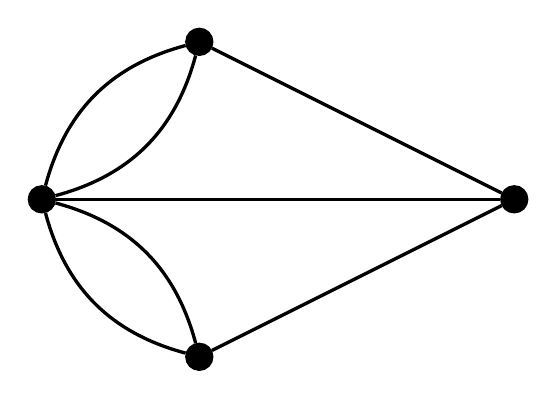
\begin{tikzpicture}
      \begin{scope}[every node/.style={circle,thick,draw=black,fill=black}]
        \node[] (A) at (0,0) {};
        \node[] (B) at (2,2) {};
        \node[] (C) at (6,0) {};
        \node[] (D) at (2,-2) {};
      \end{scope}
      \begin{scope}[every edge/.style={draw=black,very thick}]
        \path (A) edge[bend right=30] (B);
        \path (A) edge[bend left=30] (B);
        \path (A) edge[bend right=30] (D);
        \path (A) edge[bend left=30]  (D);
        \path (B) edge (C);
        \path (A) edge (C);
        \path (D) edge (C);
      \end{scope}
    \end{tikzpicture}
  \end{adjustbox}
\end{frame}

\begin{frame}{Non-deterministic Turing machine}
  \begin{description}
    \item[The usual] Turing machines are often called deterministic Turing machines.
    \item[Deterministic] Turing machines have exactly one row in their state table for every combination of (non-terminal) state and tape symbol.
    \item[This means] there is only one path to follow at a given point in time.
    \item[Nondeterministic] Turing machines can have any number of rows for each state/symbol (including none).
    \item[Essentially] they allow for parallel computation -- they can branch into two or more paths at the same time.
  \end{description}
\end{frame}


\begin{frame}{Non-deterministic Turing machine and languages}
  \begin{description}
    \item[Languages] are accepted by non-deterministic Turing machines, where an input string is accepted if any branch ends in the accept state.
    \item[Deciders] -- if a non-deterministic Turing machine always halts on all branches of computation, no matter what the input, then we say it decides the language it accepts.
    \item[Any] language that is accepted (or decided) by a non-deterministic Turing machine has some deterministic Turing machine that accepts (or decides) it. So non-deterministic Turing machines don't really have any extra abilities over deterministic ones.
  \end{description}
\end{frame}


\begin{frame}{Non-deterministic polynomial time}
  \begin{definition}
    A decision problem is in the NP complexity class if it is decidable by a non-deterministic Turing Machine in polynomial time.
  \end{definition}
  
  \begin{alertblock}{P is a subset of NP}
    Note that every determinisitic Turing machine is also a non-deterministic one, by our definitions.
    The P complexity class is a subset of NP because of this.
  \end{alertblock}

  \begin{alertblock}{Equivalent definition}
    An equivalent definition of NP that you may come across is that NP is the set of languages $A$ that can be verified in polynomial time.
    By verified we mean that a deterministic Turing machine can accept a language $\{ wc \}$ where $w$ is in $A$ and $c$ is some string, called the certificate for $w$.
  \end{alertblock}

\end{frame}